\chapter{Planificación temporal y presupuesto}

Tal y como se requiere en \cite{website:procTFG}, a lo largo de esta sección se detallarán los distintos trabajos realizados para la elaboración de este documento, siendo a su vez localizados en el tiempo. En primer lugar es preciso saber en qué elementos se descompone el trabajo realizado, para ello se empleará una descomposición en los distintos paquetes de trabajo que ha sido necesario realizar, y posteriormente se localizarán en el tiempo mediante un diagrama de Gantt. \par 

\section*{Descomposición en paquetes de trabajo}

Los distintos paquetes de trabajo se muestran en la siguiente lista: 

\begin{enumerate}

\item Fijar objetivos según las necesidades del Grupo de Investigación.

\item Determinar materiales disponibles para la realización.

\item Documentación acerca de distintos métodos de identificación de fuerzas externas.

\item Elección del método de identificación de fuerzas externas.

\item Elaboración de las ecuaciones del sistema.

\item Elaboración teórica del modelo del observador y estimador.

\item Elaboración teórica del algoritmo estimador.

\item Documentación acerca de ROS y Gazebo.

\item Familiarizarse con el modelo del Kraft existente.

\item Sustituir elemento terminal Grips por Robotiq.

\item Desarrollar plugin del Sensor Fuerza-Par.

\item Incluir modelo Sensor Fuerza-Par y Sensor IMU.

\item Desarrollar nodos de ROS para guardar datos en ficheros.

\item Desarrollar scripts de MATLAB para importar y acondicionar los datos.

\item Implementación del algoritmo estimador en MATLAB.

\item Comprobar y corregir errores en las implementaciones.

\item Ajustar parámetros del observador basado en Filtro de Kalman.

\item Realización de Ensayos para analizar el comportamiento del Estimador.

\item Redacción del documento TFG.

\item Corrección y Revisión de trabajos realizados y Documento redactado.

\item Imprimir y entregar Documento.

\end{enumerate}

\section*{Diagrama de Gantt}

En esta sección se efectuará la localización temporal de las distintas tareas mencionadas en el anterior apartado. Es preciso destacar tanto la fecha de inicio para la elaboración del \acrfull{tfg}, especificada el lunes 3 de febrero de 2014, como la fecha de finalización del mismo, que coincide con la fecha de entrega del \acrshort{tfg}, el lunes 8 de septiembre de 2014. \par 

En la figura mostrada a continuación puede observarse el diagrama de Gantt elaborado para la planificación del presente \acrshort{tfg}. En el mismo puede apreciarse un vacío, en cuanto a trabajo se refiere, de alrededor de 2 meses, en los que se puso como objetivo el estudio de los exámenes de la convocatoria ordinaria de las asignaturas matriculadas durante el curso académico 2013-2014. \par 

\newgeometry{margin=2.5cm}
\begin{landscape}
\thispagestyle{empty}
\begin{figure}[h!]
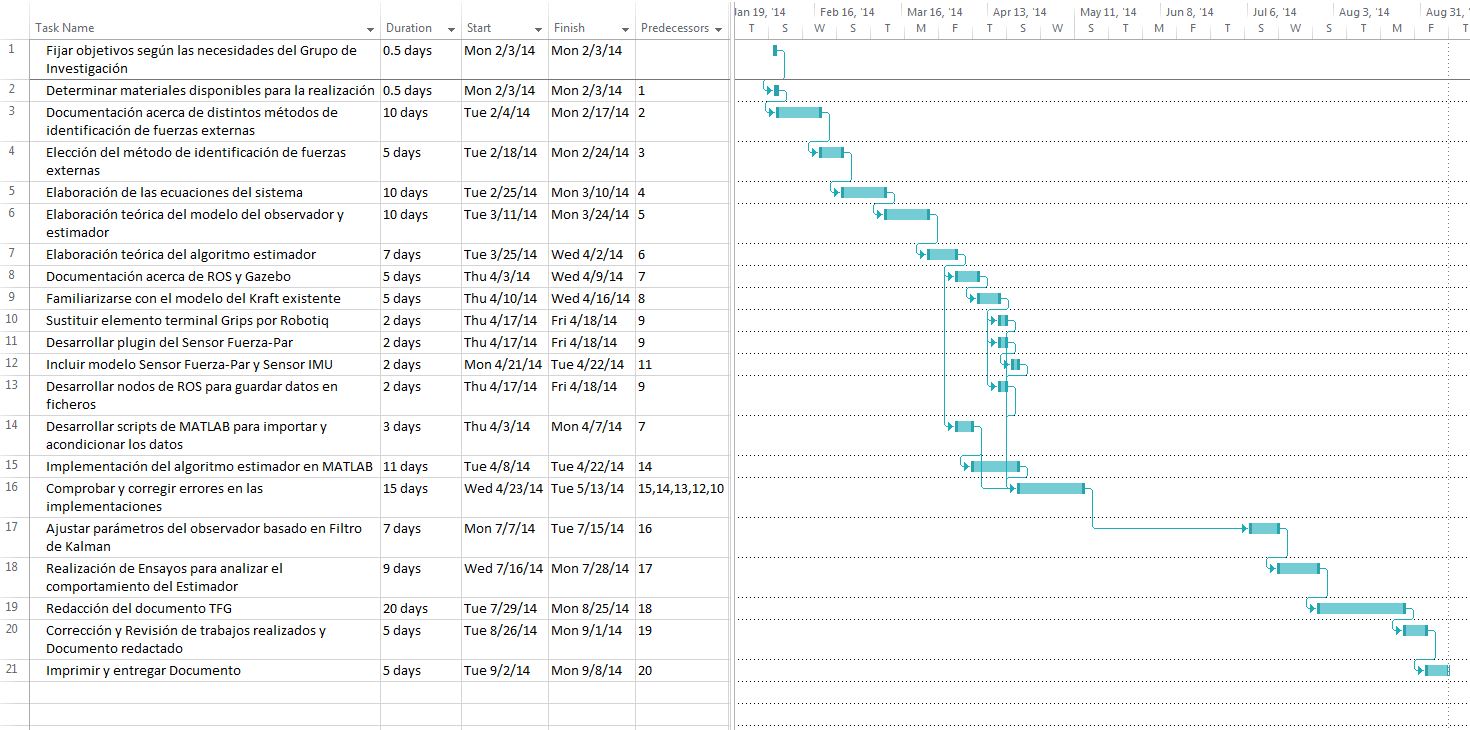
\includegraphics[width=\hsize, height=\vsize]{Figuras/Gantt}
\end{figure}
\end{landscape}
\restoregeometry

\section*{Presupuesto}

Para el cálculo del presupuesto necesitado para la realización del \acrlong{tfg} efectuado se considerarán únicamente aquellos recursos de utilización exclusiva para llevar a cabo este \acrshort{tfg}, debido a que la mayoría de equipos empleados, como el manipulador robótico de \emph{Kraft Telerobotics, Inc.} o el sensor fuerza par, son empleados por el resto de integrantes del Grupo de Investigación denominado \emph{Robots y Máquinas Inteligentes} perteneciente al \acrfull{car}, y puesto que únicamente se ha empleado el simulador Gazebo, no deben ser tenidos en cuenta en el presupuesto. \par

En la tabla mostrada a continuación, aparecen los gastos efectuados para la elaboración del \acrlong{tfg}. En ella puede apreciarse que los únicos gastos efectuados, debido a la naturaleza del trabajo, provienen del equipo necesario para efectuar las simulaciones, la licencia del programa empleado para probar el algoritmo (MATLAB) y el coste de las horas de trabajo del investigador. \par 

\begin{table}[h]
\centering
\begin{tabular}[c]{ c c c c }
\hline
\multicolumn{4}{c}{\textbf{Costes para la Realización del presente TFG}} \\
\hline
Elemento & Precio Unitario & Unidades & Coste Total \\
 & (\euro{}/ud.) & (ud.) &  (\euro{}) \\
\hline
Ordenador de Sobremesa & 1000 & 1 & 1000 \\
Licencia de MATLAB para uso académico\footnotemark & 700 & 1 & 700 \\
Recursos Humanos (Horas de Trabajo) & 20 & 300 & 6000 \\
\hline
\textbf{TOTAL} & & & \textbf{7700} \\
\hline
\end{tabular}
\caption{Coste para la Realización del presente TFG}
\end{table}

\footnotetext{Solamente se ha tenido en cuenta el precio de la licencia de MATLAB y de las distintas \emph{toolbox} empleadas para el desarrollo del trabajo (\emph{toolbox} simbólica).}